\documentclass[conference]{IEEEtran}
\IEEEoverridecommandlockouts
\usepackage{cite}
\usepackage{amsmath,amssymb,amsfonts}
% \usepackage{algorithmic}  % dropped: unused, and algorithms.sty is absent locally
\usepackage{graphicx}
\usepackage{textcomp}
\usepackage{xcolor}
\usepackage{float}
\usepackage[table]{xcolor}
\usepackage{booktabs}
\usepackage{tikz}
\usetikzlibrary{positioning,arrows.meta,calc,fit,backgrounds,shapes.geometric}
\usepackage{url}

% --------------------------------------------------------------------------
% DRAFT MARKERS.  \needswork{...} flags a gap that must be filled before
% submission; it renders as a visible red box while `draftnotes' is true and
% vanishes entirely when the flag is switched to false.  Grep for
% "needswork" to enumerate every remaining hole.
% --------------------------------------------------------------------------
\newif\ifdraftnotes\draftnotestrue
\newcommand{\needswork}[1]{%
  \ifdraftnotes\textcolor{red!75!black}{\small[\,\textbf{TODO:} #1\,]}\fi}
\newcommand{\placeholderfig}[2]{%
  \begin{tikzpicture}
    \node[draw=red!60!black, dashed, line width=.8pt, rounded corners=3pt,
          fill=red!4, minimum width=#1, minimum height=#2, align=center,
          font=\footnotesize, text=red!60!black, inner sep=6pt]
      {PLACEHOLDER FIGURE\\ (see caption for what to generate)};
  \end{tikzpicture}}

\def\BibTeX{{\rm B\kern-.05em{\sc i\kern-.025em b}\kern-.08em
    T\kern-.1667em\lower.7ex\hbox{E}\kern-.125emX}}

\begin{document}

\title{A Single Beam Is All You Need: Altimeter-Supervised Reconstruction for Under-Ice Robotic Perception}
%% Comment out for submission
% \author{
%     \IEEEauthorblockN{
%         Klára Orbán\textsuperscript{*1},
%         Ashwin Nedungadi\textsuperscript{*2},
%         Ana-Ștefania Kogălniceanu\textsuperscript{1},
%         Bianca-Marcela Sava\textsuperscript{1},
%     }
%     \IEEEauthorblockN{
%         Bastian Cieply\textsuperscript{2},
%         Raul-Alexandru Simon\textsuperscript{1},
%         Kuderna-Iulian Bența\textsuperscript{1},
%         Stefan Lüdtke\textsuperscript{2}
%     }
%     \IEEEauthorblockA{
%         \textsuperscript{1}Faculty of Mathematics \& Computer Science, Babeș-Bolyai University, Cluj-Napoca, Romania\\
%         \{klara.orban, ana.kogalniceanu, bianca.sava, raul.simon\}@stud.ubbcluj.ro,
%         kuderna.benta@ubbcluj.ro
%     }
%     \IEEEauthorblockA{
%         \textsuperscript{2}Institute of Visual \& Analytic Computing, University of Rostock, Germany\\
%         \{ashwin.nedungadi, bastian.cieply, stefan.luedtke\}@uni-rostock.de
%     }
%     \thanks{\textsuperscript{*}Equal Contribution.}
% }

\maketitle

% ===========================================================================
\begin{abstract}
Photometric 3D Gaussian Splatting (3DGS) fails on low-texture sea-ice scenes
in a systematic and previously unreported way: the photometric objective
converges to a locally consistent solution with the depth axis inverted
relative to the physical scene. On real Antarctic ROV footage from the PS117
expedition to the Weddell Sea, we show that two independent, structurally
unrelated underwater 3DGS baselines, SeaSplat and WaterSplatting, both
exhibit this failure, reaching Pearson $r = -0.234 \pm 0.771$ and
$-0.246 \pm 0.754$ respectively against a co-registered single-beam
acoustic altimeter, while reporting healthy photometric scores throughout;
training SeaSplat for $4\times$ longer does not fix it ($r=-0.259\pm0.809$).
We fix the failure by introducing the altimeter signal as a
self-diagnosing depth-supervision term during training. A stop-gradient
residual weight concentrates correction on the frames where the renderer
disagrees most with the acoustic trace, rather than discounting them as
outliers. The method requires no new hardware, since one Valeport VA500P
single-beam altimeter is already fitted to the vehicle for altitude hold,
and it adds no meaningful cost or payload relative to an imaging-sonar
alternative. On a 60\,s ROV transect under Antarctic sea ice (station
PS117-39, 298 frames, 5-fold contiguous along-track holdout), our method
reaches $r = +0.980 \pm 0.013$ and RMSE $= 0.075 \pm 0.022$\,m against
held-out altimeter pings, versus $r \approx -0.23$ to $-0.26$ and RMSE
$\approx 1.4$--$1.5$\,m for the baselines, while simultaneously attaining
the highest PSNR of the four methods compared ($36.44$\,dB). We further
show, honestly, that this correction is local rather than global. When
sonar supervision is withheld from each evaluation block during its own
training, agreement with the altimeter drops to $r = +0.425 \pm 0.516$
(RMSE $=0.463$\,m) and is sign-inverted in the block furthest from any
supervised frame, evidence that dense along-track anchoring, and not a
transferable geometric prior, is what the standard cross-validation number
measures. The trained field nonetheless yields a dense $25$\,Hz depth
trace, six times denser than the raw altimeter, suggesting a direct route
to continuous ice-draft profiling from a sensor every survey ROV already
carries.
\end{abstract}

\begin{IEEEkeywords}
Marine Robotics, Under-Ice Perception, 3D Gaussian Splatting, Acoustic-Optical
Fusion, Depth Supervision, Field Robotics
\end{IEEEkeywords}

% ===========================================================================
\section{Introduction}
% ===========================================================================

The underside of sea ice is one of the least observed surfaces on Earth, and
one of the more consequential. Its morphology governs ocean--ice heat exchange,
sets the light field available to the under-ice ecosystem, and determines
where a remotely operated vehicle can safely operate \cite{wadhams-2006,
katlein-2017}. Ice draft is a key input to ice-mass-balance models, and a dense 3D
reconstruction would also show melt-pond shapes, ridges, and where
organisms attach to the ice: none of it visible from above.
Robotic surveys are a practical way to observe this surface at
scale, and the instrument of record has long been acoustic: upward-looking
multibeam sonar mounted on an ROV or AUV recovers ice draft robustly and
independently of visibility \cite{anhaus-2024, sonar_mapping}. What acoustics
cannot recover is appearance. Albedo, transmittance, biological pigmentation
and centimetre-scale surface texture are invisible to an echosounder
and are precisely the quantities that radiative-transfer and ecosystem models
need.

Optical reconstruction is the natural complement, and the last three years
have transformed what is possible in that direction. Neural radiance fields
\cite{mildenhall2020nerf} and, more recently, 3D Gaussian Splatting
\cite{kerbl20233dgs} deliver dense, photorealistic, real-time-renderable scene
representations, and a series of underwater adaptations has made them aware of
the intervening medium: SeaThru-NeRF \cite{levy2023seathrunerf}, SeaSplat
\cite{yang2025seasplat}, WaterSplatting \cite{li2025watersplatting}, UW-GS
\cite{wang2025uwgs} and UW-3DGS \cite{xing2025uw3dgs} all model attenuation and
backscatter explicitly and report substantial gains in rendering quality on
underwater benchmarks.

These methods were developed and validated on coral reefs and man-made
structures: scenes with abundant texture and directional lighting. Sea ice
presents an opposite scenario: it is predominantly flat, and lit by diffuse under-ice
light with little directionality. We show the degrading, inversive effects of this setting on photometric 3DGS. Scored against a
co-registered single-beam altimeter on real footage from the PS117 expedition to the Weddell Sea, both SeaSplat and WaterSplatting produce rendered depth that is anti-correlated with true range, while
reporting entirely healthy photometric scores throughout training. This is not an initialisation artefact: even when MASt3R-SfM \cite{duisterhof2024mast3rsfm} supplies a correctly
oriented starting point, photometric optimisation alone corrupts it. Two independent codebases, with different SfM initialisation strategies and underwater rendering models, fail in the same way at two different stations. The consistency across implementations suggests a limitation in the objective itself rather than a fault in either codebase. This is the under-ice instance of a failure mode
increasingly recognised in the splatting literature more generally, in which
appearance metrics remain healthy while the underlying surface is wrong
\cite{huang20242dgs, guedon2024sugar}.

The failure appears to be geometric rather than radiometric. On low-texture surfaces, the photometric residual provides little information about depth, allowing different geometries to produce similar image errors. The objective therefore does not provide enough information to reliably select the correct geometry among these alternatives.
Closing that gap needs an external metric anchor, and the cheapest one available is already
on the vehicle: a single-beam altimeter, carried by essentially every ROV
and AUV for altitude hold, returning one scalar range per ping at a few
hertz. Unlike imaging-sonar fusion \cite{qadri2024aoneus, qu2024zsplat, chen2025sonarsweep},
it adds no payload, no calibration rig, and negligible cost relative to a
research ROV or camera rig.

Turning that scalar into a training signal requires care: the beam and the
camera do not always observe the same surface, and naive depth supervision
would inject error into an otherwise well-constrained reconstruction. We
therefore make the altimeter term self-diagnosing. Rather than discounting
high-residual frames as likely outliers, we invert that logic: early in training the altimeter is more reliable
than the renderer, so the frames where rendered depth disagrees most with
the acoustic trace are precisely the frames that most need correction. A
stop-gradient adaptive weight concentrates the loss accordingly.

The contributions of this paper are:
\begin{itemize}
  \item Documentation of the depth-inversion failure mode in photometric 3DGS on
   low-texture scenes, with evidence from two independent baselines and two
   independent stations.
  \item A sonar-supervised depth regularisation loss with a self-diagnosing adaptive
   weight, requiring only a single-beam altimeter.
  \item Evaluation on real sub-ice ROV data from a PS117 Weddel Sea survey, with
   5-fold contiguous along-track holdout to respect temporal autocorrelation.
  \item A dense depth trace downstream application: interpolating altimeter coverage
   from ~3.92 Hz to 25 Hz via the trained Gaussian field.
\end{itemize}

% ===========================================================================
\section{Related Work}
% ===========================================================================

\subsection{Optical Reconstruction Under and Around Ice}

Photogrammetric mapping of the ice--water interface has a short but
instructive history. Cimoli et al.\ \cite{cimoli-2019} demonstrated
hyperspectral and RGB imaging of the ice underside from a sled-mounted rig
over landfast ice, establishing that optical capture of this surface is
feasible but tightly constrained by platform geometry and illumination. ROV
platforms such as the AWI system described by Katlein et al.\
\cite{katlein-2017} carry cameras alongside their scientific payload, and
large campaigns including MOSAiC \cite{anhaus-2025-rov} have accumulated
substantial imagery, though almost always as a secondary product of surveys
designed around acoustic and bio-optical measurement rather than around
systematic photogrammetric coverage.

The consequences are well documented. Structure-from-motion in underwater
settings must contend with refraction through the port, wavelength-dependent
attenuation, and backscatter from suspended particles
\cite{qiao-2019, bryson-2015}, and dedicated seafloor-mapping work has had to
develop explicit strategies for revisiting weakly reconstructed regions
\cite{she2024seafloor}. Under ice these difficulties are sharpened by a surface
that is often genuinely featureless. Our own prior benchmark
\cite{ours-icra2026-benchmark} compared SfM against monocular depth estimation
on MOSAiC ROV data using multibeam sonar as reference, and found that neither
approach was reliable across the survey: SfM produced coherent geometry only
where image coverage and feature visibility happened to be favourable, and
monocular depth estimation \cite{lin2025depth3recoveringvisual} failed to align
with the acoustic reference at all in most regions. The follow-up study
\cite{ours-eccv2026-breakdown} localised the cause to the capture geometry
itself, showing that classical SfM \cite{schoenberger2016colmap}, 3D Gaussian
Splatting \cite{kerbl20233dgs}, TSDF fusion of monocular depth, and the
feed-forward model VGGT \cite{wang2025vggt} all fail on the same under-ice AUV
sequence, with camera baselines of only $1$--$12$\% of scene depth common to
all four. Notably, that work used altimeter returns only to invalidate a
competing image-content hypothesis, and explicitly left metric evaluation of
reconstruction accuracy against the altimeter as future work. The present
paper takes up that thread and additionally turns the altimeter from a
diagnostic into a training signal.

\subsection{Radiance Fields for Underwater Scenes}

Neural radiance fields \cite{mildenhall2020nerf} and 3D Gaussian Splatting
\cite{kerbl20233dgs} both optimise a scene representation purely against a
photometric reconstruction loss. Applied naively underwater, both misattribute
medium effects to scene radiance, and a now-substantial body of work has
addressed this by making the image formation model explicit. SeaThru-NeRF
\cite{levy2023seathrunerf} embeds the revised underwater image formation model
of Akkaynak and Treibitz \cite{akkaynak2018revised} into NeRF's volume
rendering, separating object radiance from backscatter and attenuation.
SeaSplat \cite{yang2025seasplat} carries the same physically grounded model
into 3DGS, jointly estimating medium parameters with the Gaussian scene and
recovering medium-free colour. WaterSplatting \cite{li2025watersplatting}
instead pairs an explicit Gaussian geometry with a separate volumetric field
for the scattering medium, on the argument that a purely explicit
representation cannot render the medium at all. UW-GS \cite{wang2025uwgs} adds
distance-dependent colour and a physics-based density control together with
handling for dynamic distractors; UW-3DGS \cite{xing2025uw3dgs} adds a
learnable voxel-based attenuation and backscatter module and prunes floating
Gaussians by an uncertainty criterion; and OceanSplat
\cite{kweon2026oceansplat} enforces trinocular view consistency to derive a
self-supervised depth prior. Comparative studies of these families against
refraction-aware SfM are beginning to appear \cite{muhammad-2025}.

What unites this line of work is that it improves the \emph{appearance} model
while leaving the \emph{geometric} constraint set unchanged. Each method
becomes better at explaining the observed pixels, and in a capture regime where
many distinct geometries explain those pixels equally well, that is precisely
the axis along which improvement does not help. Our results in
Section~\ref{sec:results} are consistent with this reading: the two methods we
evaluate differ substantially in how they model water, and agree almost exactly
in how badly they recover depth.

\subsection{Geometric Supervision for Radiance Fields}

That photometric optimisation alone underdetermines geometry is not specific to
underwater scenes. Deng et al.\ \cite{deng2022dsnerf} identified fitting
incorrect geometry from insufficient views as a characteristic NeRF failure
mode, observing that standard volume rendering does not enforce that scenes
consist mostly of free space and opaque surfaces, and showed that the sparse
3D points already produced by SfM serve as effectively free depth supervision.
DN-Splatter \cite{turkulainen2025dnsplatter} extends 3DGS with depth and normal
priors for exactly this reason, reporting that indoor 3DGS performs poorly
without geometric constraints during optimisation. A parallel line of work
attacks the representation rather than the loss: 2D Gaussian Splatting
\cite{huang20242dgs} collapses the volumetric primitive to an oriented disk to
remove the multi-view inconsistency of thick 3D Gaussians, and SuGaR
\cite{guedon2024sugar} regularises Gaussians toward surface alignment to permit
mesh extraction.

These methods share an assumption that does not hold in our setting: that a
dense or at least spatially distributed depth prior is available, whether from
SfM points, an RGB-D sensor, or a monocular network. Under ice, SfM points are
exactly what is missing, RGB-D sensing is not available, and monocular metric
depth is unreliable on this domain \cite{cai-2025, wu2025stereoadapteradaptingstereodepth}.
Our supervision is instead extremely sparse but physically measured: one true
metric range per frame. The question we address is whether a signal that thin
is sufficient, and, since it is not everywhere trustworthy, how to weight it.
For the latter we draw on uncertainty-based loss weighting
\cite{kendall2018uncertainty}, which learns relative task weights rather than
requiring them to be tuned by hand.

\subsection{Acoustic--Optical Fusion}

The closest work to ours fuses cameras with sonar inside a differentiable
renderer. Qadri et al.\ \cite{qadri2023neusis} reconstruct surfaces from
imaging sonar alone using a neural implicit representation with an acoustic
rendering model. AONeuS \cite{qadri2024aoneus} extends this to genuine
multimodal fusion, combining high-resolution RGB with low-resolution
depth-resolved imaging sonar, and reports accurate high-resolution surfaces
from \emph{heavily restricted baselines}, which is the same regime that defeats
the vision-only methods here. Z-Splat \cite{qu2024zsplat} frames the problem in
the language of the missing-cone artefact, noting that when surround views are
impossible the reconstruction degrades specifically along the depth axis, and
uses sonar transients to sample that axis directly. SonarSplat
\cite{sethuraman2025sonarsplat} builds a Gaussian splatting formulation for
imaging sonar itself, and SonarSweep \cite{chen2025sonarsweep} adapts plane
sweeping to cross-modal sonar--vision depth estimation. In the underwater
mapping setting, ReefMapGS \cite{yang2026reefmapgs} closes the loop between
multimodal SLAM and 3DGS, using pose-graph uncertainty to drive incremental
reconstruction.

Every one of these systems relies on a sonar that returns a
\emph{two-dimensional} acoustic image or an equivalent transient profile.
That is a strong signal and a correspondingly heavy instrument. Our claim is
narrower and, we believe, more deployable: in a capture regime whose deficiency
is one-dimensional, a one-dimensional sensor suffices. A single-beam
altimeter contributes no azimuth, no elevation and no image, only a range
along a known ray, and is already installed on the platforms that collect
polar under-ice data. To our knowledge, single-beam altimetry has not
previously been used as geometric supervision for a radiance field, and the
underwater 3DGS methods surveyed above are explicitly designed to work without
any external geometric reference.

% ===========================================================================
\begin{figure*}[t]
\centering
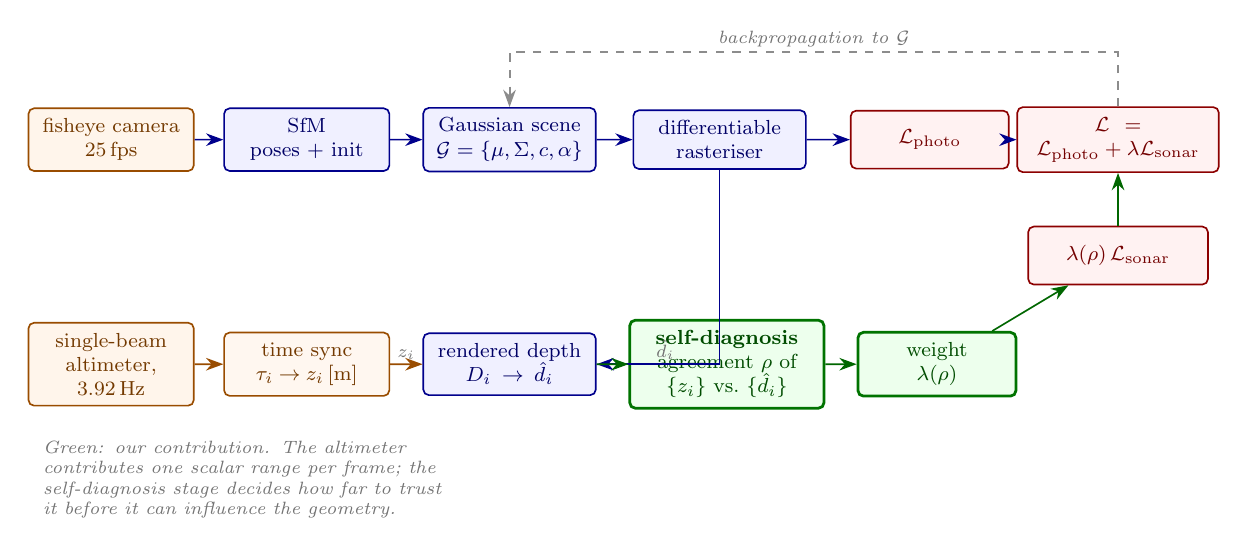
\begin{tikzpicture}[scale=0.92, transform shape,
  >={Stealth[length=2.2mm,width=1.6mm]},
  box/.style   ={draw, rounded corners=2pt, align=center, inner sep=4pt,
                 minimum height=8mm, font=\footnotesize, line width=.6pt},
  sensor/.style={box, draw=orange!60!black, fill=orange!8,  text=orange!45!black},
  vis/.style   ={box, draw=blue!55!black,   fill=blue!6,    text=blue!40!black},
  aco/.style   ={box, draw=orange!60!black, fill=orange!6,  text=orange!45!black},
  loss/.style  ={box, draw=red!55!black,    fill=red!5,     text=red!45!black},
  ours/.style  ={box, draw=green!45!black,  fill=green!7,   text=green!30!black,
                 line width=1pt},
  fl/.style    ={->, line width=.6pt, draw=blue!55!black},
  al/.style    ={->, line width=.6pt, draw=orange!60!black},
  gl/.style    ={->, line width=.6pt, draw=green!40!black},
  lbl/.style   ={font=\scriptsize\itshape, text=black!55, inner sep=1.5pt}]

  % --- vision lane -------------------------------------------------------
  \node[sensor, text width=2.0cm] (cam) at (-7.9, 1.5)
    {fisheye camera\\$25$\,fps};
  \node[vis, text width=2.0cm] (sfm) at (-5.2, 1.5)
    {SfM\\poses $+$ init};
  \node[vis, text width=2.1cm] (gs) at (-2.4, 1.5)
    {Gaussian scene\\$\mathcal{G}=\{\mu,\Sigma,c,\alpha\}$};
  \node[vis, text width=2.1cm] (rend) at (0.5, 1.5)
    {differentiable\\rasteriser};
  \node[loss, text width=1.9cm] (lp) at (3.4, 1.5)
    {$\mathcal{L}_{\text{photo}}$};

  % --- acoustic lane -----------------------------------------------------
  \node[sensor, text width=2.0cm] (alt) at (-7.9, -1.6)
    {single-beam\\altimeter, $3.92$\,Hz};
  \node[aco, text width=2.0cm] (sync) at (-5.2, -1.6)
    {time sync\\$\tau_i \!\rightarrow\! z_i\,[\mathrm{m}]$};
  \node[vis, text width=2.1cm] (dep) at (-2.4, -1.6)
    {rendered depth\\$D_i \rightarrow \hat d_i$};
  \node[ours, text width=2.4cm] (agree) at (0.6, -1.6)
    {\textbf{self-diagnosis}\\agreement $\rho$ of\\$\{z_i\}$ vs.\ $\{\hat d_i\}$};
  \node[ours, text width=1.9cm] (lam) at (3.5, -1.6)
    {weight\\$\lambda(\rho)$};

  % --- total loss --------------------------------------------------------
  \node[loss, text width=2.2cm] (ls) at (6.0, -0.1)
    {$\lambda(\rho)\,\mathcal{L}_{\text{sonar}}$};
  \node[loss, text width=2.5cm] (tot) at (6.0, 1.5)
    {$\mathcal{L}=\mathcal{L}_{\text{photo}}+\lambda\mathcal{L}_{\text{sonar}}$};

  % --- edges -------------------------------------------------------------
  \draw[fl] (cam) -- (sfm);  \draw[fl] (sfm) -- (gs);
  \draw[fl] (gs)  -- (rend); \draw[fl] (rend) -- (lp);
  \draw[fl] (lp)  -- (tot);
  \draw[al] (alt) -- (sync);
  \draw[al] (sync) -- node[lbl, above]{$z_i$} (dep);
  \draw[fl] (rend.south) |- node[lbl, pos=.72, above]{$\hat d_i$} (dep.east);
  \draw[gl] (dep) -- (agree); \draw[gl] (agree) -- (lam);
  \draw[gl] (lam) -- (ls);    \draw[gl] (ls) -- (tot);

  % backprop
  \draw[->, line width=.7pt, draw=black!45, dashed]
    (tot.north) -- ++(0,0.75) -| node[lbl, pos=.25, above]
    {backpropagation to $\mathcal{G}$} (gs.north);

  % annotation
  \node[lbl, text width=5.6cm, align=left, anchor=north west]
    at (-8.9, -2.6)
    {Green: our contribution. The altimeter contributes one scalar range per
     frame; the self-diagnosis stage decides how far to trust it before it can
     influence the geometry.};
\end{tikzpicture}
\caption{Method overview. A standard 3DGS pipeline (blue) is augmented with a
single-beam altimeter stream (orange). The rendered depth at the beam
footprint is compared against the measured range, and the agreement between the
two sequences sets the weight of the depth term, so that supervision is
asserted only where the acoustic and optical observations corroborate one
another. No additional payload is required: the altimeter is already fitted for
altitude hold.}
\label{fig:pipeline}
\end{figure*}

% ===========================================================================
\section{Problem Setting and Data}
\label{sec:data}
% ===========================================================================

We use ROV footage acquired during the PS117 expedition \cite{meiners2019polarstern} of RV Polarstern to the Weddell Sea in 2019. The primary station, PS117-39, consists of 298 fisheye video frames from a sub-ice ROV transect. The ROV travelled at approximately $0.1$,m/s, at a distance of $2$--$4$,m below the ice underside. The fisheye frames were downsampled to a width of $1600$,px. Distance to the ice underside was recorded using a Valeport VA500P altimeter at approximately $3.92$,Hz, corresponding to one measurement per $\approx 6.4$ video frames. A second station, PS117-29, contains 300 frames from the same cruise and is used as an additional dataset for comparison.

Two properties of this configuration matter for what follows. First, the
altimeter provides an independent physical measurement of range: unlike
the sparse SfM points normally used for depth supervision
\cite{deng2022dsnerf}, it does not originate from the same optical
measurements the reconstruction is fitting, so it cannot inherit their errors.
Second, it is a single narrow beam. It reports where the ice is along one ray
and says nothing about the rest of the frame.

The survey geometry is slow, the forward-dominant motion produces near-converging viewpoints and
a camera baseline that is a small fraction of scene depth, over a surface with
little usable texture. Under these conditions the photometric residual is
weakly informative about depth, and the reconstruction problem is
underdetermined in exactly the direction the altimeter measures.

\needswork{confirm the exact ROV platform, camera model, maybe add two screenshots from the videos}
% ===========================================================================
\section{Method}
\label{sec:method}
% ===========================================================================

\subsection{Background: 3D Gaussian Splatting}
\label{sec:method-init}

We build on 3D Gaussian Splatting \cite{kerbl20233dgs}, which represents a
scene as a set of anisotropic Gaussians $\mathcal{G} = \{(\mu_k, \Sigma_k,
c_k, \alpha_k)\}$ optimised by differentiable rasterisation against a
photometric objective $\mathcal{L}_{\text{photo}}$ combining $\mathcal{L}_1$
and D-SSIM terms. Depth is obtained from the same rasteriser by
$\alpha$-compositing the per-Gaussian ray depths, and is therefore a
differentiable function of the same parameters.

We initialise the Gaussians from a depth-aware point cloud produced by
applying a monocular depth model, DA3~\cite{lin2025depth3recoveringvisual}, to the training
frames. DA3 produces correctly signed monocular depth even on textureless
ice surfaces; critically, we use it only for point-cloud
initialisation, never as a training loss, so the sign-inversion analysis
below is not confounded by a monocular prior interfering with the
photometric objective during optimisation.

\subsection{Altimeter Supervised Depth Regularisation}
\label{sec:method-b}

Let $v$ denote a training view and $\hat{d}(v)$ the mean rendered depth over
a $20{\times}20$-pixel patch centred on the image plane, standing in for the
altimeter beam footprint (justified in \S\ref{sec:patch}). The altimeter
emits one pulse every $0.255$\,s; each view is matched to the temporally
nearest ping $z_s(v)$ within a $\delta = 1.0$\,s tolerance, converted to
reconstruction units as $\tilde{z}_s(v) = z_s(v)/s$, with the scale $s$
defined in \S\ref{sec:scale}.

The altimeter supervision term is
\begin{equation}
L_{\text{sonar}}(v) = w \cdot \mu(v) \cdot \left| \hat{d}(v) - \tilde{z}_s(v) \right|,
\label{eq:lsonar}
\end{equation}
with base weight $w = 0.1$ and a self-diagnosing adaptive multiplier
\begin{equation}
\mu(v) = \operatorname{clip}\!\big(1 + k \cdot |\hat{d}(v) - \tilde{z}_s(v)|_{\text{sg}},\; 0.5,\; 4.0\big),
\label{eq:mu}
\end{equation}
where $|\cdot|_{\text{sg}}$ denotes a stop-gradient: $\mu$ is computed from
the \emph{detached} residual, so it modulates the weight of
Eq.~\eqref{eq:lsonar} without itself receiving gradient. With $k = 3.0$, a
$0.1$\,m rendered-vs-sonar deviation yields $\mu = 1.3$; a $0.33$\,m
deviation saturates the ceiling at $\mu = 4.0$. The floor $\mu \geq 0.5$
prevents near-converged frames from being dominated by gradient noise. This
is the inverse of the usual robust-loss philosophy, which downweights large
residuals as likely outliers~\cite{sabour2024robustnerf}: here the altimeter is the
authority, so the most deviant rendered frames receive the strongest
correction, not the weakest.

\subsection{Scale Fitting}
\label{sec:scale}

The reconstruction's metric scale is arbitrary; we recover it with a
no-intercept least-squares fit of altimeter range on rendered depth over the
training split $T$,
\begin{equation}
s^{*} = \operatorname*{argmin}_{s} \sum_{v \in T} \left| z_s(v) - s\,\hat{d}(v) \right|^2
= \frac{\sum_{v \in T} z_s(v)\,\hat{d}(v)}{\sum_{v \in T} \hat{d}(v)^2}.
\label{eq:scale}
\end{equation}
We obtain $s^{*} = 5.24$ for PS117-39. The same fitted scale is held fixed
across all ablation variants, so that differences in $r$ and RMSE reflect geometry quality, not a
scale-fitting artefact.

\subsection{Total Objective and Texture-Aware Depth Prior}

The total training loss is
\begin{equation}
L = L_{\text{photo}} + \lambda_s\, L_{\text{sonar}} + \lambda_d\, L_{\text{depth}},
\label{eq:total}
\end{equation}
where $L_{\text{depth}}$ is an $L_1$ penalty on rendered depth against the
per-pixel DA-3 depth prior, modulated by a texture-confidence mask
$\tau \in [0,1]$ estimated from local gradient magnitude and colour variance
in the training frames. High-texture regions ($\tau \to 1$) receive full
depth regularisation; low-texture ice faces ($\tau \to 0$) receive reduced
regularisation, so the monocular prior cannot force low-confidence, flat
regions into a geometry that contradicts photometric evidence. $\tau$ is
hand-tuned on a held-out validation sequence and is not re-estimated during
training. \needswork{report $\lambda_s$, $\lambda_d$ values, optimiser and
schedule, iteration count, densification settings, and hardware/training
time -- currently only the RTX 3080 Laptop (8\,GB, $\sim$55--90\,min/model)
figure is available.}

% ===========================================================================
\section{Evaluation Protocol}
\label{sec:protocol}
% ===========================================================================

All methods are evaluated against the same independent measurements using the same procedure.

\subsection{Associating Pings with Frames}

The imagery carries no timestamps, so frame times are reconstructed
arithmetically. For a frame with index $n_i$ in the original video,
\begin{equation}
  t_i = n_i / \mathrm{fps}, \qquad \tau_i = T_0 + t_i,
\end{equation}
with $\mathrm{fps} = 25$ and $T_0$ the wall-clock time of the first video
frame. Each frame is matched to the temporally nearest altimeter ping
$k^\star(i) = \arg\min_k |t_k - \tau_i|$ and is discarded if the residual gap
exceeds $\delta = 1.0$\,s or if the ping carries the no-return sentinel. At
$3.92$\,Hz the ping period is $\approx 0.26$\,s, so $\delta$ is permissive by
construction; Section~\ref{sec:limitations} reports the sensitivity of the
results to this choice.
\needswork{run and report the $\delta$ sweep, and the distribution of realised
match gaps}

\subsection{Reducing a Render to a Comparable Scalar}
\label{sec:patch}

For each camera the depth map $D_i$ is rendered and reduced to the mean of the
central $20 \times 20$ pixels, standing in for the forward-looking beam:
\begin{equation}
  \hat d_i = \frac{1}{400}
    \sum_{|u-c_x|<10}\;\sum_{|v-c_y|<10} D_i(v,u).
\end{equation}
This assumes the beam is boresighted with
the optical axis; no sonar--camera extrinsic calibration was available
(\S\ref{sec:limitations}). Patch-size sensitivity is reported in
Table~\ref{tab:patch}.

\subsection{Scale-Free Scoring}

A monocular reconstruction is determined only up to a global scale, so a single
scale factor is fitted on a training split $\mathcal{T}$ by least squares
through the origin and then held fixed,
\begin{equation}
  s \;=\; \Big(\textstyle\sum_{i\in\mathcal{T}} z_i \hat d_i\Big)
          \Big/\Big(\textstyle\sum_{i\in\mathcal{T}} \hat d_i^{\,2}\Big).
\end{equation}
On the held-out split $\mathcal{E}$ we report Pearson correlation and RMSE,
\begin{equation}
  r = \mathrm{corr}(z, \hat d)\big|_{\mathcal{E}},
  \qquad
  \mathrm{RMSE} = \Big[\tfrac{1}{|\mathcal{E}|}
    \textstyle\sum_{i\in\mathcal{E}} (z_i - s\,\hat d_i)^2\Big]^{1/2}.
\end{equation}
The correlation $r$ is computed on the raw pairs and is therefore invariant to
$s$; it measures whether the reconstruction gets \emph{farther} as the ice gets
farther, independently of any scale convention. RMSE, in metres, is
scale-dependent and should be read as a shape-agreement residual after
scaling rather than as an absolute metric error.

\subsection{Contiguous Along-Track Holdout}

Adjacent frames on a slow-moving ROV are strongly autocorrelated, so an
interleaved every-$N$th-frame split understates error. We instead cut the
298 time-ordered PS117-39 frames into five contiguous along-track blocks of
$\approx 60$ frames each (Table~\ref{tab:folds}), hold each out in turn, and
report mean $\pm$ std across folds. For each fold, the scale $s^{*}$ is
re-fit on the training frames only and held fixed for test-time evaluation.

\begin{table}[t]
\centering
\caption{5-fold contiguous block assignment, PS117-39 (298 frames, step 5).}
\label{tab:folds}
\begin{tabular}{@{}llc@{}}
\toprule
Block & Frame range & \# frames \\
\midrule
0 & f000750--f001055 & 60 \\
1 & f001060--f001350 & 59 \\
2 & f001355--f001650 & 60 \\
3 & f001655--f001945 & 59 \\
4 & f001950--f002245 & 60 \\
\bottomrule
\end{tabular}
\end{table}

\subsection{F1: Truly Held-Out Sonar Supervision}
\label{sec:f1}

The standard cross-validation protocol above still trains on altimeter
readings from \emph{all} 298 frames -- the held-out block is excluded only
from the scale fit, not from $L_{\text{sonar}}$. To test whether sonar
supervision learns a transferable geometric prior rather than simply
anchoring the frames it directly supervises, we additionally train five
separate models, one per fold, in which the corresponding block's frames are
excluded from $L_{\text{sonar}}$ \emph{during training as well}. A frame in
the test block never contributes to the sonar loss in its own model.
This provides a stricter test of generalisation, whereas the standard CV number
in \S\ref{sec:results} represents an upper bound. Results are reported in Table~\ref{tab:f1}.

\subsection{Baselines}

\textbf{SeaSplat}~\cite{yang2025seasplat}: 3DGS with underwater appearance
modelling, trained at both $7$k (its published default) and $30$k
iterations (matched to our training budget), reported as separate rows in
Table~\ref{tab:main}. \textbf{WaterSplatting}~\cite{li2025watersplatting}:
3DGS with volumetric water-column modelling (nerfstudio), trained at its
published default. All methods are evaluated under the identical 5-fold
protocol and use the same COLMAP camera poses and dataset as our method;
neither baseline receives sonar data at any stage.

% ===========================================================================
\section{Experiments and Results}
\label{sec:results}
% ===========================================================================

\subsection{Headline Comparison}

Table~\ref{tab:main} reports geometric agreement with the altimeter alongside
photometric quality. Both baselines are not merely less accurate: their
rendered depth is anti-correlated with measured range. Two codebases with
different SfM initialisation and different water-column models land within
$0.002$ of one another, which is consistent with a shared structural cause
rather than an implementation defect in either.

\begin{table}[t]
\centering
\caption{PS117-39, 5-fold contiguous CV. Mean $\pm$ std over 5 folds.
Negative $r$ means rendered depth runs backwards against true range.}
\label{tab:main}
\resizebox{\columnwidth}{!}{%
\begin{tabular}{@{}lccc@{}}
\toprule
Method & PSNR $\uparrow$ & Sonar $r$ $\uparrow$ & Sonar RMSE $\downarrow$ \\
\midrule
WaterSplatting~\cite{li2025watersplatting} & 30.24\,dB & $-0.246\pm0.754$ & $1.416\pm0.387$\,m \\
SeaSplat~\cite{yang2025seasplat} (7k) & 21.75\,dB & $-0.234\pm0.771$ & $1.460\pm0.397$\,m \\
SeaSplat (30k) & \needswork{missing} & $-0.259\pm0.809$ & $1.451\pm0.418$\,m \\
\textbf{Ours} (sonar-supervised, 30k) & \textbf{36.44\,dB} & \textbf{$+0.980\pm0.013$} & \textbf{$0.075\pm0.022$}\,m \\
\bottomrule
\end{tabular}%
}
\end{table}

Our method also attains the highest PSNR of the three despite carrying an
additional loss term, indicating that on this data the geometric constraint
does not compete with photometric quality but is consistent with it.

\subsection{Ablations}

Table~\ref{tab:ablation} isolates the contribution of sonar supervision
from the DA-3 initialisation and texture-confidence weighting, and
separately isolates the adaptive weighting scheme (Eq.~\eqref{eq:mu}) from
sonar supervision itself. The no-sonar variant is positive on average
($r = +0.398 \pm 0.647$) but the standard deviation is large enough that
individual folds still land on the wrong side of zero: DA-3 initialisation
and texture-confidence weighting alone \emph{help} but do not
\emph{guarantee} correct sign, which is why sonar supervision is still
doing real work and not merely polishing an already-correct
reconstruction. The fixed-weight variant ($k{=}0$ in Eq.~\eqref{eq:mu},
i.e.\ $\mu \equiv 1$) currently measures $r = +0.985 \pm 0.011$, RMSE
$= 0.064$\,m, close to the full adaptive weighting's
$r = +0.980 \pm 0.013$, RMSE $= 0.075$\,m.

\begin{table}[t]
\centering
\caption{Ablations on PS117-39, 5-fold contiguous CV.}
\label{tab:ablation}
\resizebox{\columnwidth}{!}{%
\begin{tabular}{@{}lccl@{}}
\toprule
Variant & Sonar $r$ & Sonar RMSE \\
\midrule
No sonar (DA-3 + $\tau$ only) & $+0.398\pm0.647$ & $0.487$\,m \\
Fixed weight ($\mu{\equiv}1$) & $+0.985\pm0.011$ & $0.064$\,m \\
Full adaptive ($k{=}3.0$) & $+0.980\pm0.013$ & $0.075$\,m \\
\bottomrule
\end{tabular}%
}
\end{table}

\needswork{PENDING VERIFICATION -- do not treat the fixed-vs-adaptive comparison
above as settled. Before drawing any conclusion from it: (1) rerun both
variants to rule out a run-to-run fluke or a bug in the fixed-weight
implementation; (2) test statistical significance (e.g.\ paired across
folds) rather than eyeballing overlapping std-devs; (3) only after that,
decide whether the paper's framing of adaptive weighting as the mechanism
needs to change. One plausible account, if the gap holds up, is that
PS117-39's altimeter returns are uniformly clean at $3.92$\,Hz with no
dropped or spurious pings, leaving little disagreement for an adaptive
scheme to exploit -- the dropout sweep below directly tests whether
adaptive weighting earns its complexity once the altimeter trace is
noisier.}

\subsection{F1: Held-Out Sonar Supervision}

\begin{table}[t]
\centering
\caption{F1 experiment: one model per fold, sonar withheld from that fold's
own frames during training (\S\ref{sec:f1}). Train $r$ confirms the model
converged on its supervised frames; Test $r$ is the honest generalisation measure.}
\label{tab:f1}
\begin{tabular}{@{}lccc@{}}
\toprule
Fold & Test $r$ (held out) & Test RMSE & Train $r$ (saw sonar) \\
\midrule
0 & $-0.396$ & $0.377$\,m & $+0.994$ \\
1 & $+0.666$ & $0.466$\,m & $+0.996$ \\
2 & $+0.979$ & $0.572$\,m & $+0.960$ \\
3 & $+0.055$ & $0.469$\,m & $+0.947$ \\
4 & $+0.820$ & $0.430$\,m & $+0.958$ \\
\midrule
\textbf{F1 aggregate} & $\mathbf{+0.425\pm0.516}$ & $\mathbf{0.463\pm0.064}$\,m & --- \\
Std.\ CV (upper bound) & $+0.980\pm0.013$ & $0.075\pm0.022$\,m & --- \\
\bottomrule
\end{tabular}
\end{table}

The gap between standard CV ($r = +0.980$) and F1 aggregate ($r = +0.425$)
reveals that sonar supervision anchors geometry \emph{locally} but does not
propagate globally. Block~2 (middle segment, surrounded by supervised
frames on both sides) holds at $r = +0.979$ held-out. Block~0 (first
segment, no upstream supervised frames at all) sign-inverts. Block~3
collapses to near-zero despite being a middle segment; this likely reflects
a scene geometry transition at that transect position.

\begin{figure}[htbp]
\centering
\placeholderfig{7.2cm}{4.4cm}
\caption{Rendered depth against measured altimeter range on the held-out
block, one point per frame, for all three methods with their fitted regression
lines. This is the figure that carries the central claim and it must be plotted
from the actual per-frame pairs; a schematic must not be substituted.}
\label{fig:signflip}
\end{figure}

\begin{figure}[htbp]
\centering
\placeholderfig{7.2cm}{3.6cm}
\caption{Qualitative comparison: a rendered novel view and the corresponding
depth map for each method, with the closest and farthest altimeter readings in
the sequence shown alongside for reference.}
\label{fig:qualitative}
\end{figure}

\subsection{Sensitivity Analysis}

\textbf{Patch size} (Table~\ref{tab:patch}): correlation is stable
($0.975$--$0.980$) across $10$--$40$\,px patches; RMSE rises at $40$\,px as
larger patches average over off-axis regions of the fisheye field of view,
justifying the $20{\times}20$\,px default.

\begin{table}[t]
\centering
\caption{Sensitivity to altimeter-patch size, PS117-39.}
\label{tab:patch}
\begin{tabular}{@{}lcc@{}}
\toprule
Patch size & Sonar $r$ & Sonar RMSE \\
\midrule
$10{\times}10$\,px & $0.977 \pm 0.013$ & $0.085 \pm 0.021$\,m \\
$20{\times}20$\,px (default) & $\mathbf{0.980 \pm 0.013}$ & $\mathbf{0.075 \pm 0.022}$\,m \\
$40{\times}40$\,px & $0.975 \pm 0.016$ & $0.134 \pm 0.044$\,m \\
\bottomrule
\end{tabular}
\end{table}

\textbf{Ping rate} (Table~\ref{tab:pingrate}): performance degrades
substantially from $3.92$\,Hz to ${\sim}1.0$\,Hz (RMSE $3.5\times$
higher), then plateaus: ${\sim}0.2$\,Hz and ${\sim}0.1$\,Hz yield
virtually identical results. Sign flips appear in blocks~0 and~3 at
the sparse rates regardless of exact duty cycle, echoing the F1 locality
finding. At ${\sim}1.0$\,Hz ($r=+0.843$) correct-sign geometry is still
recovered across all folds.

\begin{table}[t]
\centering
\caption{Ping-rate sweep, PS117-39.}
\label{tab:pingrate}
\begin{tabular}{@{}lcc@{}}
\toprule
Ping rate & Sonar $r$ & Sonar RMSE \\
\midrule
$3.92$\,Hz (full) & $+0.987\pm0.010$ & $0.063$\,m \\
${\sim}1.0$\,Hz (every 4th) & $+0.843\pm0.101$ & $0.223$\,m \\
${\sim}0.2$\,Hz (every 20th) & $+0.370\pm0.569$ & $0.448$\,m \\
${\sim}0.1$\,Hz (every 40th) & $+0.374\pm0.570$ & $0.493$\,m \\
\bottomrule
\end{tabular}
\end{table}

\textbf{Sonar dropout} (Table~\ref{tab:dropout}): all five blocks maintain
positive $r$ at every dropout level, including $75\%$ ($r=+0.807\pm0.125$,
RMSE $=0.303$\,m). Degradation is monotone and gradual, suggesting the
method tolerates realistic altimeter outages without catastrophic failure.

\begin{table}[t]
\centering
\caption{Random sonar dropout sweep, PS117-39.}
\label{tab:dropout}
\begin{tabular}{@{}lcc@{}}
\toprule
Dropout & Sonar $r$ & Sonar RMSE \\
\midrule
$0\%$ & $+0.974\pm0.027$ & $0.085$\,m \\
$25\%$ & $+0.953\pm0.033$ & $0.116$\,m \\
$50\%$ & $+0.900\pm0.051$ & $0.178$\,m \\
$75\%$ & $+0.807\pm0.125$ & $0.303$\,m \\
\bottomrule
\end{tabular}
\end{table}

\subsection{Dense Depth Trace}
\label{sec:dense-trace}

The trained Gaussian field enables rendering depth at every video frame, not just at frames matched to a sonar ping. We run the trained model (ours, 30k, full ping rate) over all 298 PS117-39 frames and match each rendered depth to the nearest ping for evaluation, while keeping unmatched frames as the dense interpolation product.

\begin{table}[t]
\centering
\caption{Dense depth trace: rendered depth at full 25 Hz video rate vs. the sparse altimeter.}
\label{tab:dense}
\begin{tabular}{@{}lcc@{}}
\toprule
 & Dense trace (ours) & Raw altimeter \\
\midrule
Rate & $25.0$\,Hz & $4.98$\,Hz \\
Frames & 298/300 & 298/300 \\
Sonar $r$ & $+0.995$ & --- \\
Sonar RMSE & $0.077$\,m & --- \\
\bottomrule
\end{tabular}
\end{table}

At matched frames the dense trace achieves $r = +0.995$, RMSE $= 0.077$\,m (Table~\ref{tab:dense}), a slightly higher correlation than the cross-validation headline ($r = +0.980$) because here the scale is fit on the full 298 frames without any holdout. The effective depth-profile rate is $25$\,Hz vs.\ the raw altimeter's $4.98$\,Hz: a $5\times$ densification. This suggests a direct path to continuous ice-draft profiling from sensors every survey ROV already carries.

% ===========================================================================
\section{Discussion}
% ===========================================================================

\subsection{Why the Sign Inverts}

Under a narrow baseline the photometric residual is nearly flat along the depth
axis, the missing-cone regime described by Qu et al.\ \cite{qu2024zsplat}. The
optimiser is then free to satisfy the observed images with a family of
geometries, of which the correct one is only a member. On a low-texture surface
under a range-coupled light source, nothing in the objective distinguishes
``surface receding'' from ``surface approaching, with compensating radiance'',
and gradient descent from an SfM initialisation that is itself weakly
constrained may settle on either. The two baselines settling on the same wrong
branch is what makes the case that this is a property of the objective and the
capture geometry, not of a particular implementation.

\subsection{Why One Beam Suffices}

The deficiency is one-dimensional: what the images fail to fix is the depth
axis. A single-beam altimeter measures exactly that axis, in metric units,
independently of the optical channel. It cannot describe the surface, but it
does not need to; it needs only to select the correct member of the family the
photometric loss cannot separate. This is why a sensor several orders of
magnitude less informative than an imaging sonar
\cite{qadri2024aoneus, qu2024zsplat} can nonetheless close the gap, and it is
also why we would expect the benefit to shrink as baselines widen.

\subsection{Limitations}
\label{sec:limitations}

\textbf{Single scene.} Every number reported here comes from one survey
window at one station. Two independent baselines failing identically is
evidence against an implementation fault, but both consumed the same scene and
the same initialisation, so the scene itself remains a confound.

\textbf{Sensor geometry is assumed, not calibrated.} The central-patch reduction
presumes the beam is boresighted with the optical axis and treats a fixed pixel
window as a beam footprint, on a fisheye image where angular subtense varies
across the field. No sonar--camera extrinsic calibration was available.
\needswork{state whether extrinsics were ever measured}

\textbf{Scaled RMSE.} The reported RMSE follows a fitted scale and therefore
measures shape agreement rather than absolute metric accuracy. The unfitted
residual, which is the quantity that would demonstrate metric correctness, is
not yet reported.

\textbf{Evaluation depth definitions differ.} The three pipelines expose
rendered depth differently, with only some applying $\alpha$-normalisation.
Since $r$ is scale-free the sign result is unaffected, but the RMSE column
inherits this inconsistency.

\subsection{Toward Deployment}
\needswork{ICRA reviewers will ask what the improved geometry enables. Add a
downstream demonstration, for example ice-draft profiling against the
altimeter, a collision-margin estimate, or a localisation improvement, together
with runtime, memory and a statement of onboard feasibility}

% ===========================================================================
\section{Conclusion}
% ===========================================================================

Vision-only 3D reconstruction of the sea-ice underside does not fail gracefully.
On real Antarctic ROV footage, two state-of-the-art underwater Gaussian
splatting methods recover depth that runs backwards against a measured
altimeter trace, while their photometric metrics give no indication that
anything is wrong. Because the capture regime leaves the depth axis
underdetermined, no refinement of the appearance model can be expected to fix
this; an external metric reference is required. We have shown that the
reference does not need to be an expensive one. A single-beam altimeter, one
scalar range per ping from an instrument already fitted to essentially every
survey vehicle, is sufficient to recover correctly signed and
well-correlated geometry when introduced as a self-diagnosing depth term,
without sacrificing rendering quality. Extending the evaluation across stations,
ablating the adaptive weighting against a fixed one, and demonstrating a
downstream navigation or science task remain the immediate next steps.

% ===========================================================================
\section*{Acknowledgment}
% ===========================================================================
\needswork{update the acknowledgement for PS117: the workshop-paper text
thanked the MOSAiC team and AWI, which applies only if MOSAiC data is also
used here. Add the correct expedition, grant and data-provider acknowledgements
for the PS117 material}

\bibliographystyle{IEEEtran}
\bibliography{references}

\end{document}
